% Chapter Template
%\usepackage{subfig}
\chapter{Estado del Arte} % Main chapter title

\label{Chapter2} % Change X to a consecutive number; for referencing this chapter elsewhere, use \ref{ChapterX}

%----------------------------------------------------------------------------------------
%	SECTION 1
%----------------------------------------------------------------------------------------

\section{An\'alisis de im\'agenes de la retina}

En el mundo hay aproximadamente 285 millones de personas con discapacidad visual, de las cuales 39 millones son ciegas y 246 millones presentan baja visi\'on. Aproximadamente un 90\% de la carga mundial de discapacidad visual se concentra en los pa\'ises de ingresos bajos.
El 82\% de las personas que padecen ceguera tienen 50 años o m\'as. En t\'erminos mundiales, los errores de refracci\'on no corregidos constituyen la causa m\'as importante de discapacidad visual, pero en los pa\'ises de ingresos medios y bajos las cataratas siguen siendo una de las principales causantes de ceguera. El n\'umero de personas con discapacidades visuales atribuibles a enfermedades infecciosas ha disminuido considerablemente en los \'ultimos 20 años. Del total mundial de casos de discapacidad visual, el 80\%  se pueden evitar o curar.

Con arreglo a la Clasificaci\'on Internacional de Enfermedades (CIE10, actualizaci\'on y revisi\'on de 2006), la funci\'on visual se subdivide en cuatro niveles:
\begin{itemize}
\item visi\'on normal.
\item discapacidad visual moderada.
\item discapacidad visual grave.
\item ceguera.
\end{itemize}
La discapacidad visual moderada y la discapacidad visual grave se reagrupan com\'unmente bajo el t\'ermino “baja visi\'on”, la baja visi\'on y la ceguera representan conjuntamente el total de casos de discapacidad visual. En general, si tenemos alg\'un problema en la transparencia de los medios del ojo, la luz ya no podr\'a llegar al cerebro en las condiciones \'optimas para ver, y tendremos una discapacidad visual.
Entre el 5 y el 15\% de ellas no tiene tratamiento. En estos casos, la detecci\'on y estimulaci\'on precoz, la adaptaci\'on de ayudas para baja visi\'on o la terapia visual pueden ser tratamientos que mejoren mucho la funci\'on visual residual.

La distribuci\'on mundial de las principales causas de discapacidad visual es la siguiente:
\begin{itemize}
\item errores de refracci\'on (miop\'ia, hipermetrop\'ia o astigmatismo) no corregidos: 43\%.
\item cataratas no operadas: 33\%.
\end{itemize}
Y existe un orden para las tres enfermedades principales que causan ceguera a nivel mundial:
\begin{itemize}
\item Retinopat\'ia Diab\'etica.
\item Glaucoma.
\item Degeneraci\'on Macular asociada a la edad.
\end{itemize}
Aproximadamente un 90\% de la carga mundial de discapacidad visual se concentra en los pa\'ises en v\'ias de desarrollo. Alrededor de un 65\% de las personas con discapacidad visual son mayores de 50 años, si bien este grupo de edad apenas representa un 20\% de la poblaci\'on mundial. Con una poblaci\'on anciana en aumento en muchos pa\'ises, m\'as personas estar\'an en riesgo de sufrir discapacidad visual por enfermedades oculares cr\'onicas y envejecimiento.
A su vez se estima que el n\'umero de niños con discapacidad visual asciende a 19 millones, de los cuales 12 millones la padecen debido a errores de refracci\'on, f\'acilmente diagnosticables y corregibles. Unos 1,4 millones de menores de 15 años sufren ceguera irreversible y necesitan intervenciones de rehabilitaci\'on visual para su pleno desarrollo psicol\'ogico y personal.
En los \'ultimos 20 años, en t\'erminos generales, las tasas mundiales de discapacidad visual han disminuido desde comienzos de los años noventa. Ello pese al envejecimiento de la poblaci\'on en el mundo entero. Esa disminuci\'on se debe principalmente a la reducci\'on del n\'umero de casos de discapacidad visual por enfermedades infecciosas.
En este \'ambito organizaciones como la OMS, se centran en reforzar los esfuerzos desplegados a nivel nacional y de pa\'ises para la eliminaci\'on de la ceguera evitable, ayudar a los dispensadores nacionales de atenci\'on sanitaria a tratar las enfermedades oculares, ampliar el acceso a los servicios oftalmol\'ogicos y expandir las intervenciones de rehabilitaci\'on para personas con discapacidad visual residual. Se otorga especial importancia a la creaci\'on y el fortalecimiento de los sistemas de salud. El decenio estar\'a centrado en la creaci\'on de sistemas de salud accesibles e integrales.

La retina es una capa de tejido en la parte posterior del ojo que percibe la luz y env\'ia las im\'agenes al cerebro. En el centro de este tejido nervioso se encuentra la m\'acula. La cual provee la capacidad de enfoque central y la agudeza necesaria para leer, conducir y ver en forma clara los detalles. Las enfermedades de la retina afectan este importante tejido, afectando la vista y algunas son lo suficientemente graves como para causar ceguera. Algunos ejemplos son:
\begin{itemize}
\item Degeneraci\'on macular: Enfermedad que destruye la agudeza de la visi\'on central.
\item Retinopat\'ia diab\'etica del ojo.
\item Glaucoma.
\item Desprendimiento de retina: Urgencia m\'edica que ocurre cuando la retina se despega de la parte posterior del ojo.
\item Retinoblastoma: C\'ancer de la retina. Es m\'as com\'un en niños pequeños.
\item Membrana epirret\'inica: Tejido cicatricial en la m\'acula.
\item Agujero macular: Pequeña ruptura en la m\'acula que suele ocurrir en personas mayores de 60 años.
\item Cuerpos flotantes: Telarañas o pequeñas manchas en el campo de la vista.
\end{itemize}
Las enfermedades de la retina son la principal causa de discapacidad visual. Es preciso abordar la exposici\'on a los factores de riesgo y realizar ex\'amenes oculares peri\'odicos que permitan un diagn\'ostico precoz de la enfermedad y un tratamiento oportuno para evitar o retrasar la  disminuci\'on de la funci\'on visual. Hasta el 80\% de los casos de discapacidad visual y ceguera en adultos son prevenibles o tratables. En los pa\'ises de ingresos bajos y medios-bajos la mayor\'ia de los casos de discapacidad visual son prevenibles o curables. Para lograr una reducci\'on sustancial es preciso informar al p\'ublico general acerca de las medidas de prevenci\'on. El sistema de atenci\'on de salud debe incluir servicios de oftalmolog\'ia con el fin de alcanzar la cobertura sanitaria universal.

El an\'alisis de im\'agenes de la retina es de gran importancia para la detecci\'on de enfermedades tanto visuales como sist\'emicas.
El avance tecnol\'ogico ha permitido obtener im\'agenes de la retina de mayor calidad, lo que contribuye a mejorar su an\'alisis y permite la detecci\'on precoz de enfermedades con mayor precisi\'on, favoreciendo la disminuci\'on del porcentaje de personas con ceguera prevenible. 

Existen muchas ventajas en el uso del an\'alisis de imagen digital para cuantificar la existencia o gravedad de diferentes enfermedades vasculares, principalmente en lo que refiere a la detecci\'on temprana de retinopat\'ia diab\'etica, degeneraci\'on macular asociada a la edad,  glaucoma, hipertensi\'on arterial, entre otras.
Mediante la teleoftalmolog\'ia o la telemedicina en combinaci\'on con la asistencia de una computadora o dispositivo, se puede realizar el an\'alisis de comunidades alejadas de zonas urbanas o situadas en zonas de riesgo, permitiendo identificar a individuos que padezcan alguna patolog\'ia retinal, en una etapa temprana, a modo de prevenci\'on. \cite{kanagasingam2014progress}

Durante la \'ultima d\'ecada, la fotograf\'ia digital a color ha sido reconocida como una modalidad aceptable para documentar el aspecto de la retina, ya que proporciona informaci\'on vital sobre su estado. La segmentaci\'on y el an\'alisis de im\'agenes de la retina es de gran utilidad ya que facilita la detecci\'on de riesgos patol\'ogicos o da\~nos, y asistir en el diagn\'ostico de enfermedades. 
El avance en la tecnologia aplicada en las imagenes digitales y  el aumento de la potencia de c\'alculo de los dispositivos de procesamiento digital, ofrecen la posibilidad de utilizar estas tecnolog\'ias en oftalmolog\'ia. 
T\'ecnicas de procesamiento de imágenes, análisis y visión a traves de dispositivos computacionales se encuentran hoy en d\'ia en todos los campos de la ciencia m\'edica. Estas técnicas son especialmente relevantes para la oftalmología moderna, un campo que depende en gran medida de los datos visuales. Las im\'agenes de la retina son ampliamente utilizadas por ofatalm\'ologos para fines de diagn\'ostico. Sin embargo, estas im\'agenes a menudo necesitan mejoras visuales antes de determinar un an\'alisis digital de riesgo patol\'ogico o la detecci\'on de da\~nos. 
(Lo anterior referencia a -> Marrugo2011)
Actualmente existen diversas \'areas de investigación activas en lo que respecta a la imagenología de la retina. Algunas de estas \'areas se centran en la b\'usqueda de herramientas rentables, f\'aciles de usar y portables, que asistan en el an\'alisis y procesamiento de las im\'agenes.


En esta secci\'on describiremos en detalle la anatom\'ia del ojo, las enfermedades que usualmente se manifiestan a trav\'es de cambios en la retina, realizando una breve descripci\'on de las tres principales causantes de ceguera prevenible a nivel mundial. Tambi\'en se realizara un an\'alisis de las modalidades m\'edicas que permiten la observaci\'on de la retina, realizando hincapi\'e en las im\'agenes de fondo de ojo explicando su importancia, modo de captura, ventajas y desventajas que ofrece esta modalidad con respecto a otras, y que enfermedades se pueden detectar mediante el uso de esta modalidad.
%-----------------------------------
%	SUBSECTION 1
%-----------------------------------
\subsection{Introducci\'on}

La estructura anatómica del ojo se compone básicamente por la córnea (transparente), la esclera (normalmente blanca), el iris (que da color al ojo) y la pupila. Todas estas partes son visibles desde el exterior, y son las responsables de permitir la visión: un rayo de luz pasa a través de la córnea, que enfoca parcialmente la imagen, luego pasa por la cámara anterior, la pupila (que hace las veces de lente y enfoca aún más la imagen), la vítrea y por último es enfocado en la retina. La retina es un tejido en capas que recubre el interior del ojo, y es el encargado de la conversi\'on de la luz entrante en señales neuronales adecuadas para su posterior procesamiento por parte de la corteza visual del cerebro.
La retina posee la siguiente estructura macrosc\'opica:
\begin{itemize}
\item El disco \'optico, papila \'optica o punto ciego es una zona circular situada en el centro de la retina, por donde salen del ojo los axones de las c\'elulas ganglionares de la retina que forman el nervio \'optico. Esta \'area mide 1.5 x 2.5 mm en el ojo humano y carece de sensibilidad a los est\'imulos luminosos por no poseer ni conos ni bastones, ello causa una zona ciega dentro del campo visual que se conoce como punto ciego. Dentro de la papila se encuentra una excavaci\'on fisiol\'ogica llamada c\'upula. El cociente entre el di\'ametro de la c\'upula y el di\'ametro del disco \'optico (\'indice normal es menor a 0,3) es un indicador del daño que origina el glaucoma. El nervio \'optico de un ojo humano normal est\'a formado por los axones de entre 1 y 1,2 millones de neuronas que transportan la informaci\'on visual desde la retina hasta el cerebro. En donde las señales son procesadas e interpretadas por el cerebro.
\item La m\'acula: se puede ver como una mancha amarilla localizada en la retina. La macula o f\'ovea es la especializada en la visi\'on fina de los detalles, es donde se concentran la mayor cantidad de conos y bastones. Entre otras cosas, nos sirve para poder leer y distinguir las caras de las personas. Se localiza en la parte posterior de la retina y tiene una extensi\'on aproximada de 5 mm de di\'ametro.
\item Vasos sangu\'ineos: La retina posee un gran n\'umero de vasos sangu\'ineos encargados de tranportar la sangre y oxigenar el ojo. Cuando en un determinada zona del ojo, los niveles del flujo de sangre y de oxigeno son bajos, se produce una sustancia que provoca un crecimiento de los vasos sangu\'ineos, llevando mas oxigeno a la zona.
\end{itemize}
La microvasculatura retinal es \'unica, ya que es la \'unica parte del sistema circulatorio humano que puede ser visualizado directamente y de forma no invasiva in vivo. Permitiendo fotografiar f\'acilmente el ojo, permitiendo el an\'alisis de las im\'agenes digitales.  \cite{patton2006retinal}

\begin{figure}[H]
	{
	\centering
	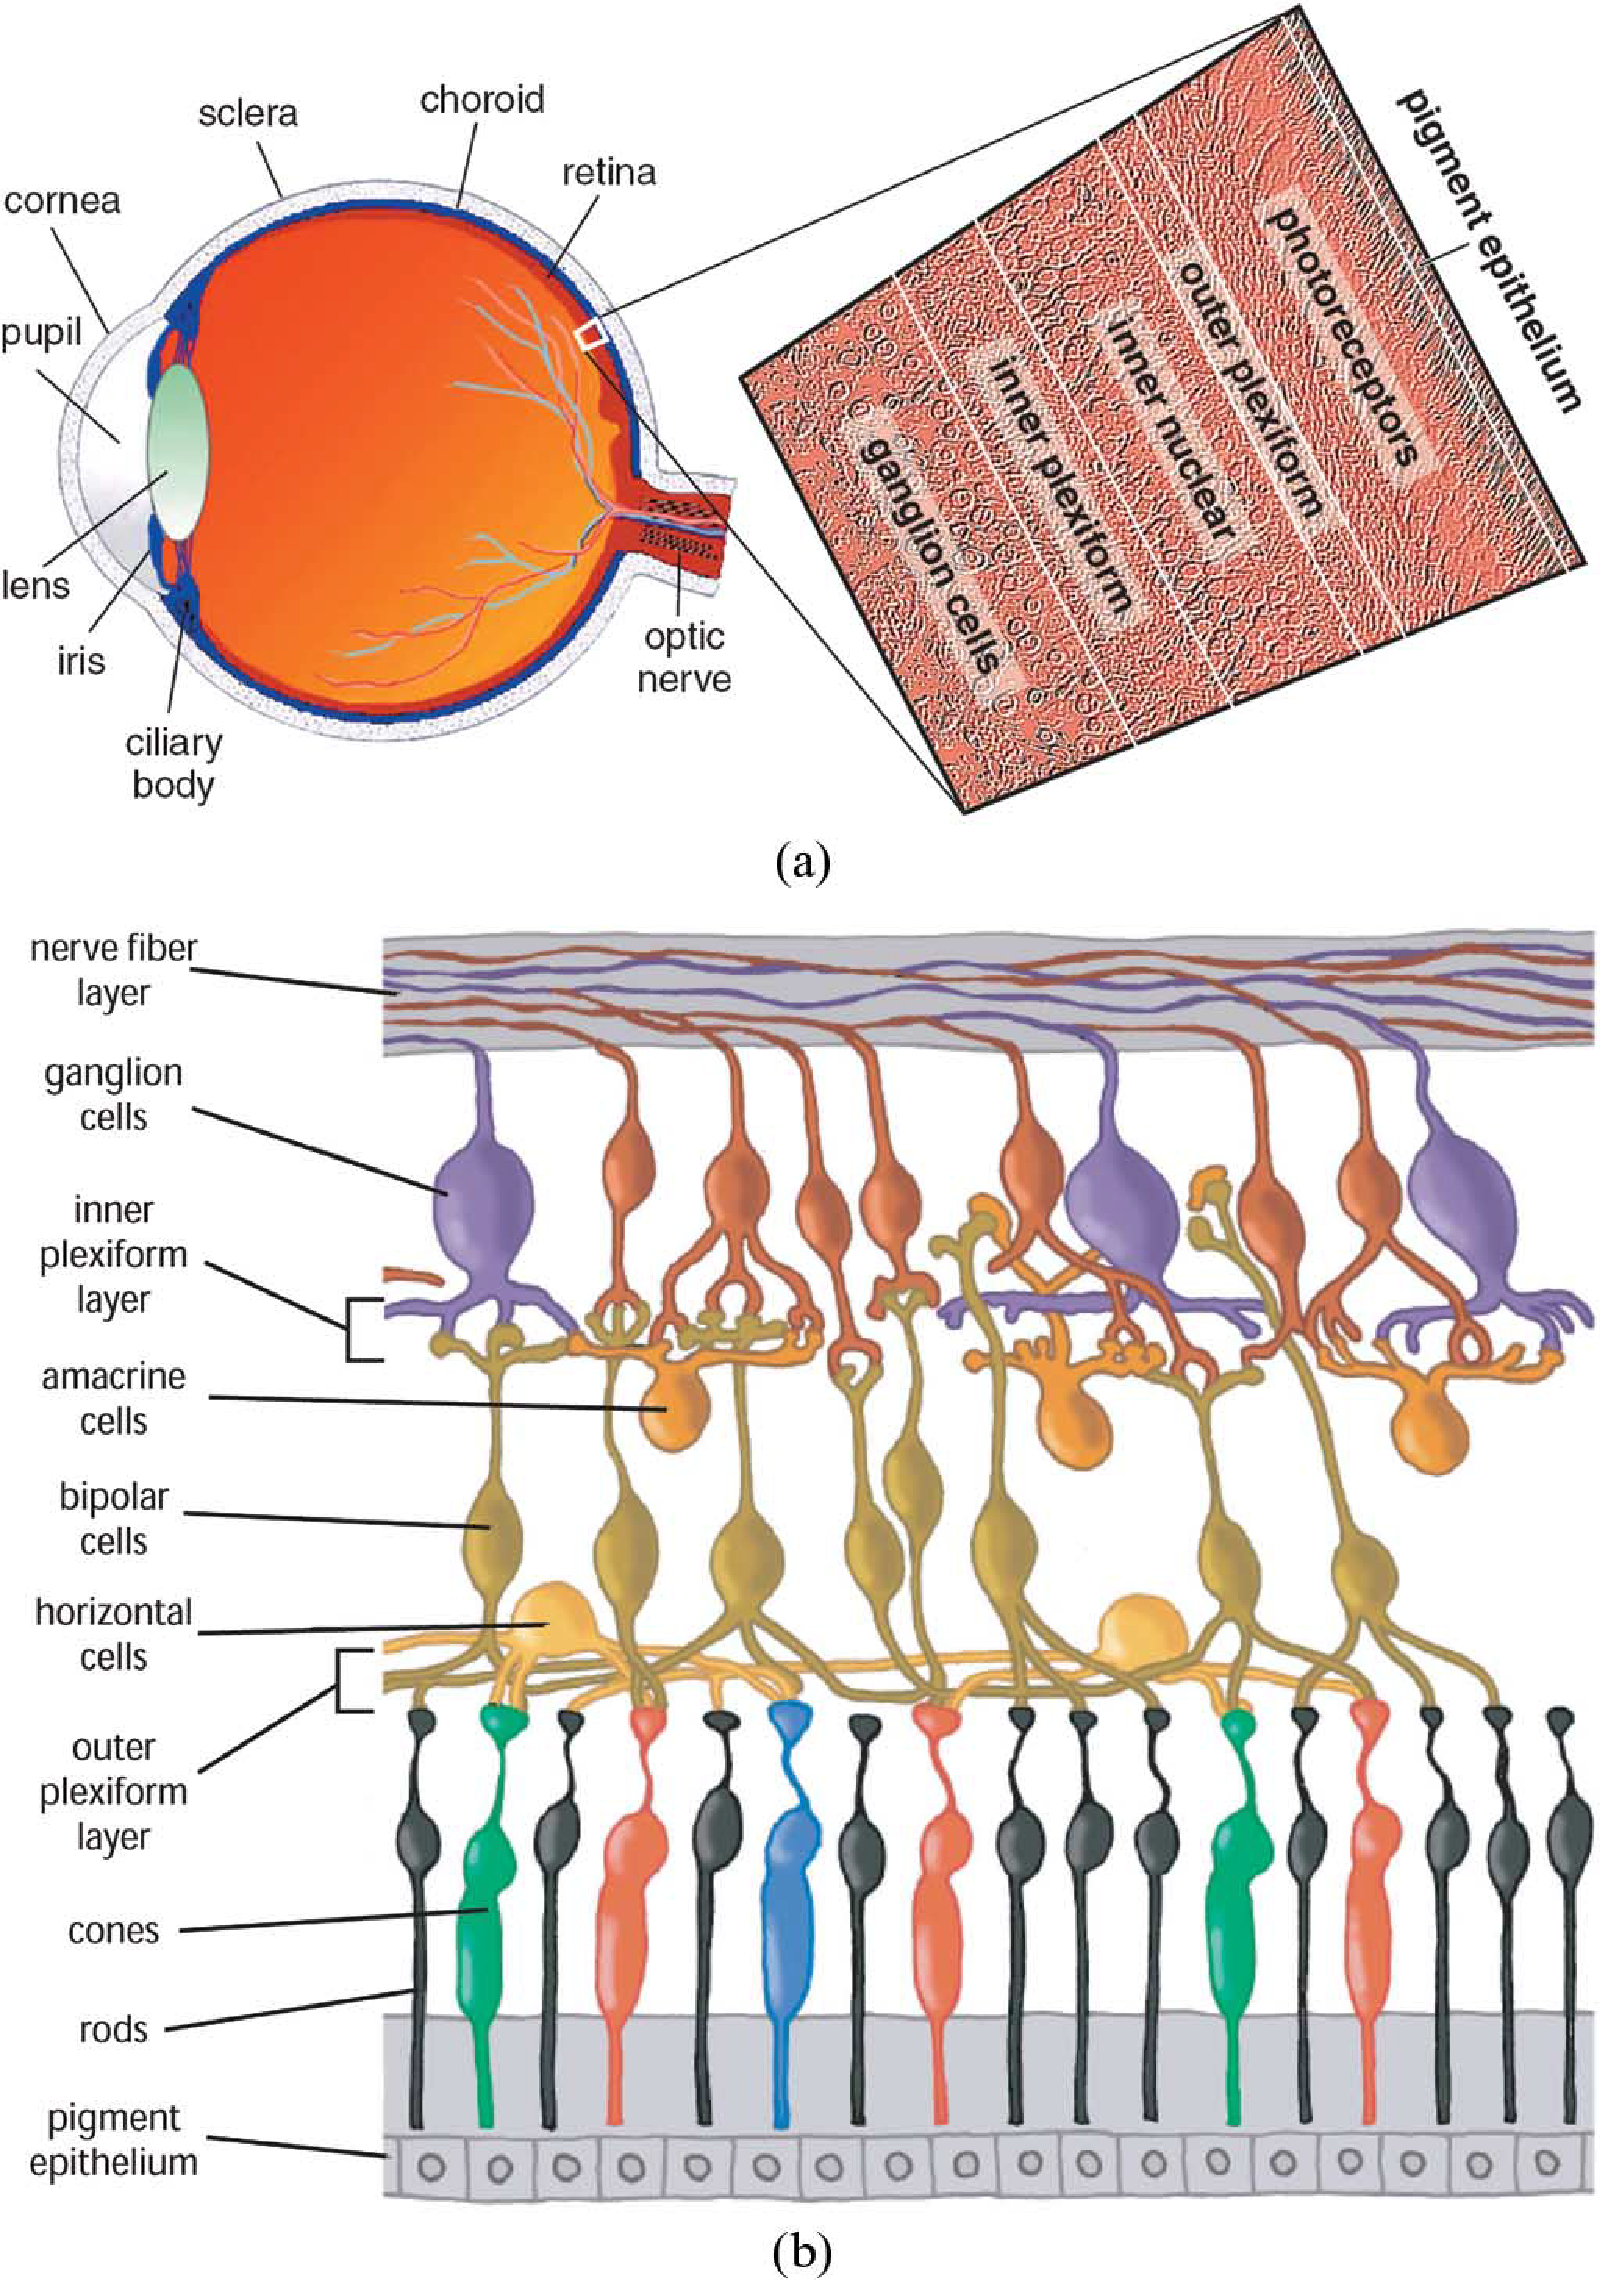
\includegraphics[width=0.75\textwidth]{Figures/ojo}
	\caption[Anatom\'ia del ojo 0-200]{\'Anatom\'ia del ojo. Ilustraci\'in de la anatom\'ia del ojo y capas de la retina [2], [3]. (A) Vista transversal del ojo y sus estructuras principales. La retina es un tejido delgado transparente que recubre la parte posterior del ojo y se compone de un n\'umero de capas, como se ilustra en la parte ampliada. (B) Representaci\'on esquem\'atica de las capas celulares de la retina. (a) Ilustraci\'on bidimensional de la anatom\'ia del ojo. (b)Representaci\'on esquem\'atica de las capas de la retina. Ejemplos de Kolb [3] utilizado con el permiso de Sigma Xi, The Scientific Sociedad de Investigación, Research Triangle Park, Carolina del Norte.}
	\label{fig:AnatomiaDelOjo}
	}
\end{figure}	

Las enfermedades que pueden manifestarse en el ojo pueden ser b\'asicamente de dos tipos, visuales o sist\'emicas, dependiendo de si ocurren en la retina misma o en el cerebro o el sistema cardiovascular, respectivamente. Algunas de estas enfermedades pueden ser f\'acilmente detectadas utilizando im\'agenes de las distintas estructuras que componen la retina.
\begin{itemize}
	\item \textbf{La retinopat\'ia diab\'etica} es una complicaci\'on ocular de la diabetes, producida por el deterioro de los vasos sangu\'ineos que irrigan la retina del fondo de ojo,  y afecta a un tercio de los diab\'eticos  y es la principal causa de p\'erdida de visi\'on en personas de edad avanzada,  y sigue siendo una de las principales causas de ceguera evitable. Estos vasos sangu\'ineos alterados pueden sufrir un debilitamiento de su pared y permitir la salida de l\'iquido o sangre, provocando el crecimiento de ramificaciones fr\'agiles en forma de cepillo, y sufrir oclusiones (trombosis). Cuando la sangre o l\'iquido que sale de los vasos daña la retina, la imagen enviada al cerebro se hace borrosa. La permeabilidad vascular y la deposici\'on de exudados duros en la retina central, puede desarrollarse en cualquier etapa de la DR y aflige a 21 millones de personas en el mundo.  A trav\'es de ex\'amenes peri\'odicos de la vista, la p\'erdida de la visi\'on relacionada con la diabetes se puede prevenir en el 98\% de los casos. (Lo anterior referencia a -> g0h2016)
 Hay dos tipos de retinopat\'ia diab\'etica. 
\begin{enumerate}
	\item Retinopat\'ia no proliferativa: En ella los vasos sangu\'ineos localizados dentro de la retina presentan cambios; algunos disminuyen de tamaño y otros se agrandan y forman sacos o dilataciones en forma de globo que entorpecen u obstruyen la circulaci\'on de la sangre. Estos vasos sangu\'ineos gotean y sufren hemorragias. El suero en el tejido fuera de los vasos produce hinchaz\'on de la retina, es lo que t\'ecnicamente se conoce como edema retiniano. Cuando el edema se reabsorbe quedan l\'ipidos atrapados en el tejido, estos depósitos se llaman exudados.
La retinopatía no proliferativa est\'a considerada como etapa inicial de la retinopat\'ia diab\'etica. Afortunadamente en un 80\% de los casos la afectaci\'on de la retinopatía no produce una perdida acusada de la visi\'on. En algunos pacientes, los exudados mencionados pueden acumularse en la zona central de la retina (m\'acula). En estos casos la perdida de visi\'on puede ser considerable. La retinopat\'ia no proliferativa es una señal de peligro, ya que puede avanzar a etapas m\'as graves y dañar la vista.
\begin{figure}[H]
	{
	\centering
	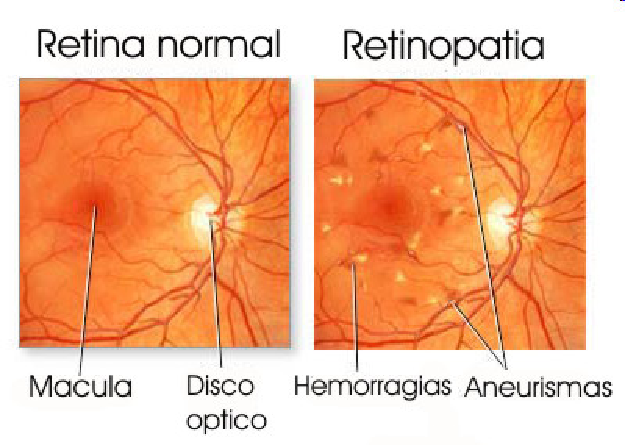
\includegraphics[width=0.5\textwidth]{Figures/Retinopatia}
	\caption[Retinopatia]{Retinopatia}
	\label{fig:Retinopatia}
	}
\end{figure}
\item Retinopat\'ia proliferativa. Este tipo comienza de la misma manera que la no proliferativa pero, en su evoluci\'on hay un fen\'omeno de isquemia (falta de aporte oxigenado a las c\'elulas). La isquemia hace que el tejido estimule la formaci\'on de vasos sangu\'ineos en un intento desesperado de recuperar el aporte sangu\'ineo, y se produce neoformaci\'on de vasos sangu\'ineos en la superficie de la retina o del nervio \'optico. Estos vasos sangu\'ineos neoformados, tienen una gran fragilidad, pueden romperse y sangrar dentro del humor v\'itreo, que es la sustancia transparente y gelatinosa que llena el centro del globo ocular. Si la sangre oscurece el humor v\'itreo que normalmente es transparente, se bloquea la luz que pasa hacia la retina, y las im\'agenes se ven distorsionadas. Adem\'as, el tejido fibroso que se forma a partir de la masa de los vasos sangu\'ineos rotos en el humor v\'itreo puede estirar y retraer la retina, desprendi\'endola del fondo del ojo. Los vasos sangu\'ineos pueden tambi\'en formarse en el iris y causar un aumento de la presi\'on ocular, dando lugar a severas p\'erdidas de la visi\'on.
\begin{figure}[H]
	{
	\centering
	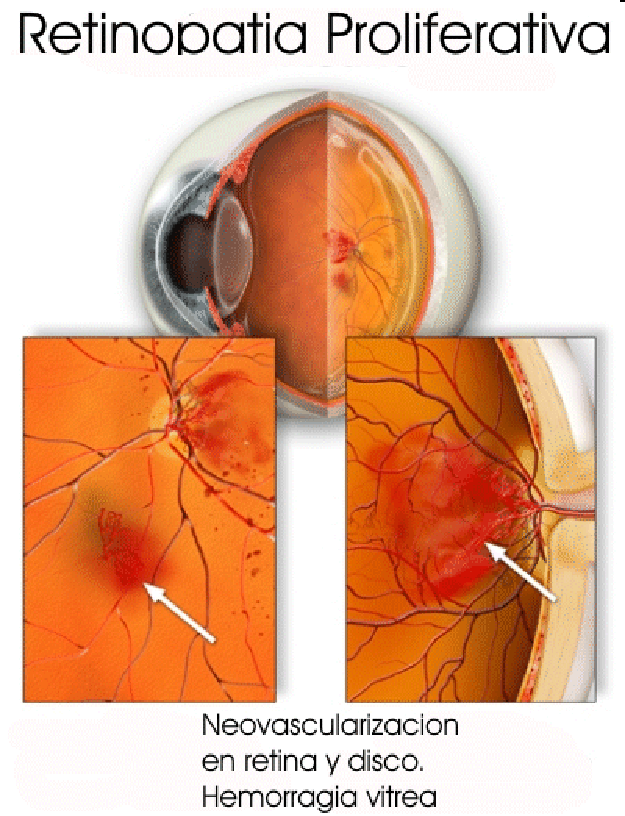
\includegraphics[width=0.5\textwidth]{Figures/RetinopatiaPrliferativa}
	\caption[Retinopatia Proliferativa]{Retinopatia Proliferativa}
	\label{fig:RetinopatiaProliferativa}
	}
\end{figure}
\end{enumerate}
La retinopat\'ia diab\'etica presenta las siguientes estructuras patol\'ogicas asociadas:
\begin{itemize}
	\item Los microaneurismas son, como su nombre sugiere, pequeñas dilataciones saculares. Los oftalm\'ologos saben que, si bien se presentan en varios procesos patol\'ogicos como hipertensi\'on, oclusi\'on venosa y alteraciones hemorreol\'ogicas, son caracter\'isticos de la retinopat\'ia diab\'etica. Su importancia se acent\'ua por el hecho de que son el primer signo cl\'inicamente identificable de la retinopat\'ia diab\'etica no proliferativa, por lo que la detecci\'on de microaneurismas puede representar un primer paso para la prevenci\'on secundaria de la evoluci\'on de la retinopat\'ia diab\'etica a la fase proliferativa y a la consiguiente p\'erdida de la visi\'on grave.
\item La hemorragia v\'itrea es la existencia de sangre en una zona del interior del ojo que se llama humor v\'itreo o cuerpo v\'itreo. El humor v\'itreo es una sustancia gelatinosa y transparente que ocupa 2/3 del volumen total del ojo, y est\'a formado por agua en un 99\%. Limita en su parte posterior con la retina y en su porci\'on anterior con el cristalino y el cuerpo ciliar. Si se produce una hemorragia en el humor v\'itreo, \'este pierde su transparencia y la luz no puede atravesarlo, lo que ocasiona p\'erdida de visi\'on.
\item	Exudados:
\begin{itemize}
	\item Dep\'ositos lip\'idicos retinianos (exudados duros). Son dep\'ositos intrarretinianos de l\'ipidos y prote\'inas, de color amarillo o blanquecinos, brillantes y bordes circulares bien definidos. Cuando se encuentran en la zona de la m\'acula adoptan forma de estrella (estrella macular) que es un signo de disminuci\'on de la agudeza visual, aunque pueden adquirir m\'ultiples formas y localizarse en otras zonas de la retina. Aparecen como consecuencia de un aumento de permeabilidad vascular por isquemia prolongada o bien tras reabsorci\'on de edemas o hemorragias retinianas. 
\item Manchas isqu\'emicas retinianas profundas (Infiltrados algodonosos o exudados blandos) Son manchas blanquecinas, difusas, de bordes mal definidos y de un di\'ametro similar a la papila. Estan principalmente en la capa nerviosa de la retina, generalmente en el polo posterior, b\'asicamente en la distribuci\'on de los capilares retinales radiales peripapilares. Suelen asociarse a microaneurismas.
\end{itemize}
\end{itemize}

\item \textbf{Degeneraci\'on macular asociada a la edad (DMAE)}, es la causa mas frecuente de ceguera en pa\'ises desarrollados en personas mayores de 50 anos. En la poblaci\'on mundial de 2002, m\'as de 161 millones de personas padec\'ian alguna discapacidad visual; de todas ellas, 124 millones ten\'ian disminuci\'on de la agudeza visual y 37 millones sufr\'ian ceguera,  de estos la degeneraci\'on macular senil afecta al 8,7\%. Una de las principales medidas para definir la gravedad de la DMAE, es el an\'alisis de derrames, alteraciones pigmentarias, atrofia geogr\'afica  y neovascularizaci\'on coroidea. Esta patolog\'ia se asocia con la edad, es m\'as frecuente en personas de raza blanca, en mujeres, cuando existen antecedentes familiares, en pacientes con hipercolesterolemia y en fumadores. La enfermedad causa lesiones en la porci\'on central de la retina llamada m\'acula. \'Esta es la responsable de la visi\'on central, necesaria para leer o conducir. La degeneraci\'on macular puede ser:
\begin{itemize}
	\item Seca o atr\'ofica: Constituye el 85\% de todos los casos. Presenta una evoluci\'on lenta a lo largo del tiempo (años). La degeneraci\'on macular seca se produce cuando las c\'elulas de la m\'acula sensibles a la luz se van deteriorando poco a poco haciendo que la visi\'on central se nuble gradualmente en el ojo afectado. A medida que la degeneraci\'on macular seca empeora, se puede observar un punto borroso en el centro de la visi\'on. Con el tiempo, cuando menos de la m\'acula funciona, es posible que se pierda progresivamente la visi\'on central en el ojo afectado. El s\'intoma m\'as com\'un de la degeneración macular seca es tener la vista un poco borrosa. La degeneraci\'on macular seca generalmente afecta ambos ojos, pero se puede perder la vista en un ojo mientras que el otro ojo parece no estar afectado. Una de las primeras señales m\'as comunes de la degeneraci\'on macular seca son las drusas. Las drusas son dep\'ositos amarillos debajo de la retina. Frecuentemente se encuentran en las personas mayores de 60 años. La degeneraci\'on macular seca tiene tres etapas, todas pueden ocurrir en uno o en ambos ojos:
\begin{enumerate}
	\item La degeneraci\'on macular temprana. Las personas con degeneraci\'on macular temprana tienen varias drusas pequeñas o algunas drusas medianas. En esta etapa, no hay s\'intomas ni p\'erdida de visi\'on.
\item La degeneraci\'on macular intermedia. Las personas con degeneraci\'on macular intermedia tienen muchas drusas de tamaño mediano, o una o m\'as drusas grandes. Algunas personas ven un punto borroso en el centro de su visi\'on. Es posible que necesiten m\'as luz para leer y para realizar otras tareas.
\item La degeneraci\'on macular seca avanzada. Adem\'as de las drusas, las personas con degeneraci\'on macular seca avanzada tienen un deterioro de las c\'elulas sensibles a la luz y del tejido de apoyo en el \'area central de la retina. Este deterioro puede causar un punto borroso en el centro de su visi\'on. Con el tiempo, el punto borroso puede agrandarse y obscurecerse, opacando m\'as su visi\'on central. Si por causa de la degeneraci\'on macular seca se tiene una p\'erdida de visi\'on en un solo ojo, es posible que no se perciba ning\'un cambio en la visi\'on en general, mientras que el otro ojo vea con claridad. Solamente  se notar\'a cambios en la visi\'on si la degeneraci\'on macular afecta a ambos ojos. 
\end{enumerate}	
\item	H\'umeda o exudativa: Se caracteriza por presentar nuevas formaciones de vasos sangu\'ineos que crecen debajo de la m\'acula. Estos vasos constituyen la denominada membrana neovascular. Su evoluci\'on es r\'apida (d\'ias/semanas) y compromete severamente la visi\'on central.
No produce dolor, pero puede presentar una serie de s\'intomas visuales que el paciente debe reconocer: las l\'ineas rectas que pueden parecer onduladas o entrecortadas, la estimaci\'on de las distancias y las alturas puede estar alterada, la sensibilidad a la luz puede estar aumentada y la necesidad de una mayor cantidad de luz para leer. Puede existir visi\'on borrosa en la parte central de la visi\'on, adem\'as cuando la enfermedad se halla en una fase m\'as avanzada puede verse una mancha negra en la zona central de la visi\'on, pudi\'endose hacer m\'as oscura y de mayor tamaño cuanto mayor tiempo de evoluci\'on tenga. Los tratamientos actuales para la DMAE no pueden curar o revertir la p\'erdida de la visi\'on. Sin embargo, el estudio de las enfermedades oculares relacionadas con la edad, mostr\'o que la suplementaci\'on con vitamina antioxidante espec\'ifica reduce el riesgo de progresi\'on de etapas intermedias, siendo una estrategia preventiva en pacientes correctamente identificados. De este modo la identificaci\'on temprana de pacientes con DMAE es importante para diseñar e implementar estrategias preventivas para el tratamiento del DMAE, y determinar su relaci\'on coste-eficacia.
\end{itemize}
\item \textbf{Glaucoma} Como se menciono anteriormente, m\'as de 161 millones de personas padecen alguna discapacidad visual; de ellas 37 millones sufr\'ian ceguera,  y de estos el glaucoma afecta al 12,3\%. Los factores de riesgo de glaucoma bien definidos son la edad avanzada, los antecedentes familiares de glaucoma, la presi\'on intraocular elevada, la utilizaci\'on de corticoides, los traumatismos oculares y otras patolog\'ias oftalmol\'ogicas predisponentes. Entre estos factores de riesgo, el \'unico que en la actualidad se puede modificar es la presi\'on intraocular alta. El aumento de la presi\'on en el ojo ocurre como resultado de la acumulaci\'on de l\'iquido en el globo ocular. 
El nervio \'optico est\'a constituido por los axones que provienen del sistema nervioso central, lugar en el que pierden la mielina y se reparten por toda la retina. En la secci\'on donde se encuentra el disco  \'optico se presenta una pequeña depresi\'on central (excavaci\'on) fisiol\'ogica, que no debe superar el tercio del tamaño total de la papila.  Cuando existe un aumento de la presi\'on del ojo, esta depresi\'on fisiol\'ogica se hace mayor.
\begin{figure}[H]
	{
	\centering
	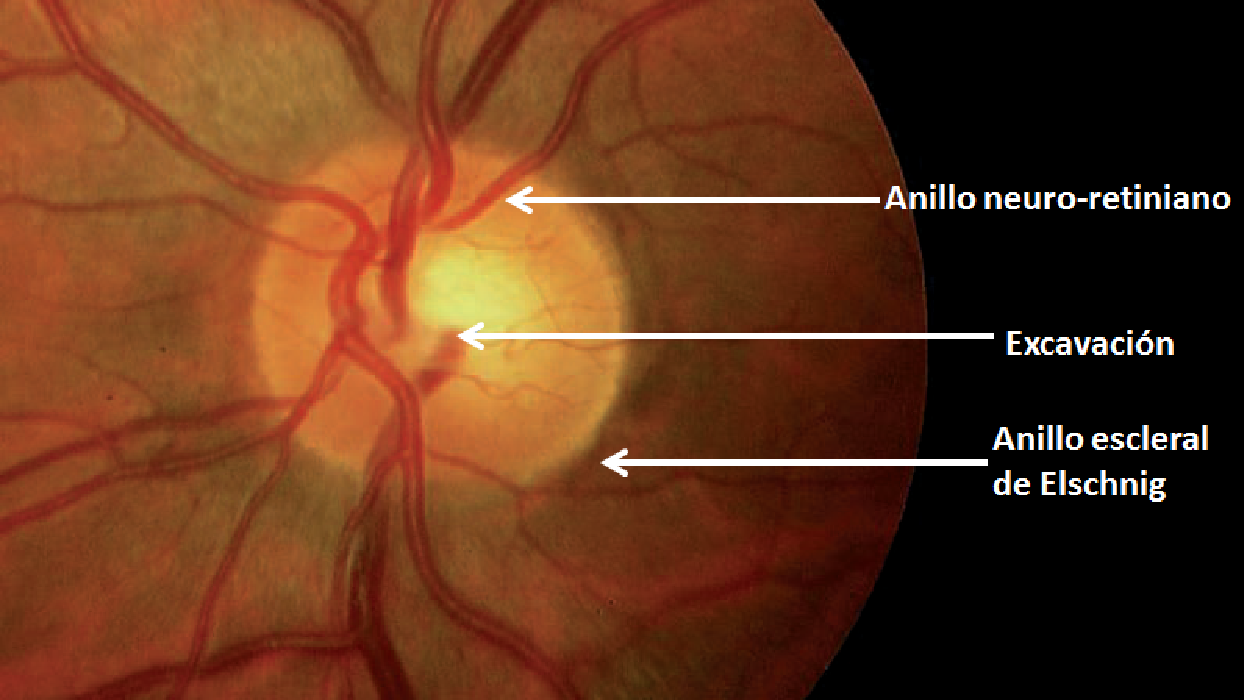
\includegraphics[width=0.5\textwidth]{Figures/nervioOptico}
	\caption[Glaucoma]{Partes del nervio \'optico}
	\label{fig:Glaucoma}
	}
\end{figure}
El l\'iquido alimenta el ojo y lo mantiene sano. Despu\'es de que el l\'iquido circula \'este se vac\'ia a trav\'es de un desagüe en la parte frontal del ojo. En las personas con glaucoma el desagüe en el ojo est\'a bloqueado y el l\'iquido no puede salir del globo ocular. En vez de esto, el l\'iquido se acumula y ocasiona un aumento de la presi\'on en el ojo. 
La parte frontal del ojo est\'a llena de un l\'iquido claro llamado humor acuoso, el cual es producido constantemente en la parte posterior del ojo. Este l\'iquido sale del ojo a trav\'es de canales en la c\'amara frontal de \'este y finalmente va al torrente sangu\'ineo. Los canales que drenan el humor acuoso est\'an en un \'area llamada el \'angulo de la c\'amara anterior o simplemente el \'angulo. El glaucoma de \'angulo cerrado (agudo) es causado por un cambio en la posici\'on del iris del ojo que s\'ubitamente bloquea la salida del humor acuoso. Esto provoca una elevaci\'on r\'apida, severa y dolorosa en la presi\'on dentro del ojo (presi\'on intraocular). El glaucoma de \'angulo cerrado es una situaci\'on de emergencia y difiere mucho del glaucoma de \'angulo abierto, el cual daña la visi\'on en forma lenta e indolora. Si una persona ha tenido glaucoma agudo en un ojo, est\'a en riesgo de un ataque en el segundo ojo, y es probable que el m\'edico recomiende un tratamiento preventivo. Las gotas para dilatar los ojos y ciertos medicamentos sist\'emicos pueden desencadenar un ataque de glaucoma agudo si la persona est\'a en riesgo. El glaucoma cong\'enito con frecuencia se da en familias (hereditario). Est\'a presente al momento de nacer y es el resultado del desarrollo anormal de los canales colectores de l\'iquido en el ojo. En el glaucoma de \'angulo abierto, la causa es esencialmente desconocida. Un aumento en la presi\'on ocular ejerce presi\'on sobre la uni\'on del nervio \'optico y la retina en la parte posterior del ojo, reduciendo el suministro de sangre al nervio \'optico. El glaucoma secundario es causado por: 
•	Medicamentos como los corticosteroides.
•	Enfermedades oculares como la uve\'itis.
•	Enfermedades sist\'emicas.
No hay cura para el glaucoma pero puede ser controlado. El tratamiento inmediato en la primera etapa puede ayudar a proteger la p\'erdida de la visi\'on. Los tratamientos suelen incluir gotas para los ojos y/o cirug\'ia. La trascendencia de cualquier enfermedad est\'a en funci\'on de su gravedad y prevalencia. En el caso del glaucoma, la gravedad viene determinada por el hecho de que su evoluci\'on natural es hacia la ceguera, y en cuanto a su prevalencia se estima en un 2 \% de la poblaci\'on mayor de 40 años. El glaucoma es el causante de entre 10 y 15 \% de la ceguera mundial, y representa la segunda causa de ceguera en pa\'ises en desarrollo.
Cambios en el nervio \'optico:
\begin{itemize}
	\item Reducci\'on del grosor del anillo neuro-retiniano.
	\item Crecimiento de la depresi\'on central o excavaci\'on.
	\item Asimetr\'ia interocular de la excavaci\'on del disco \'optico.
	\item Defectos de capa de fibras nerviosas: En sujetos normales, las fibras temporales inferiores son m\'as visibles que las superiores, \'estas que las nasales superiores y, por \'ultimo, las nasales inferiores. Las fibras temporales-maculares son las m\'as delgadas y, por tanto, las menos visibles. Una violaci\'on de esta regla puede servir tambi\'en como gu\'ia para detectar p\'erdidas difusas o focales amplias.
	\item Hemorragias del anillo neuro-retinal.
	\item Vasos sangu\'ineos con ramificaci\'ones irregulares, se presentan vasos con dos ángulos de $90^{\circ}$, en forma de valloneta.
\end{itemize}
\end{itemize}
 
A partir de la proyecci\'on de im\'agenes de fondo de ojo, la tomograf\'ia de coherencia \'optica (OCT) y otras modalidades. Cada una de estas modalidades de imagen tienen puntos fuertes y puntos d\'ebiles para detectar, capturar y / o cuantificar diferentes patolog\'ias.
A continuaci\'on se describir\'an de los tres m\'etodos m\'as comunes, el m\'etodo de captura, elementos necesarios, si son o no invasivas al organismo y su costo.
\begin{itemize}
	\item Fondo de ojo: Para realizar la captura del fondo de ojo, se dilata la pupila con f\'armacos que se depositan en forma de gotas en la superficie ocular; as\'i, el oftalm\'ologo puede ver con facilidad el interior del globo ocular con un aparato que se llama oftalmoscopio. El oftalmoscopio consiste en un aparato formado por una serie de espejos y cristales que alumbran la retina del ojo sin que la luz se refleje. Si no fuese por el oftalmoscopio la luz provocar\'ia destellos y no se podr\'ia ver el fondo de ojo de manera correcta, algo parecido a lo que sucede cuando el flash de una c\'amara de fotos saca los ojos en color rojo. Esta modalidad no es invasiva, y su costo es menor a la angiograf\'ia y la OCT dado que la cámara que se necesita para capturar la imagen del ojo es una c\'amara digital convencional.
\item Angiograf\'ia Fluorescente: Se le administrar\'an gotas oculares que hacen dilatar la pupila. Se debe colocar la barbilla sobre un apoya-ment\'on y la frente contra una barra de soporte para mantener la cabeza quieta durante el examen. Se tomar\'an fotograf\'ias del interior del ojo. Despu\'es de tomar el primer grupo de im\'agenes, se inyecta un tinte llamado fluoresce\'ina, dentro del  torrente sangu\'ineo. En la mayor\'ia de los casos, se inyecta en la parte interior del codo. Un dispositivo similar a una c\'amara toma fotograf\'ias a medida que el tinte va pasando a lo largo de los vasos sangu\'ineos en la parte posterior del ojo. Esta modalidad es invasiva dado que requiere la inyecci\'on de  un tinte fluorescente en el organismo, y es m\'as costoso debido a que se requiere un dispositivo que capte la fluorescencia generada por el tinte inyectado.
\item Tomograf\'ia de coherencia \'optica (OCT, por sus siglas en ingles): El OCT es una t\'ecnica de imagen tomogr\'afica \'optica, no invasiva, que permite visualizar tejidos oculares con un nivel de resoluci\'on microm\'etrico, diez veces mayor que al alcanzado por t\'ecnicas ultrasonogr\'aficas. Esto permite apreciar cambios sutiles de los diferentes tejidos del ojo casi a nivel celular, permiti\'endonos entender mejor los procesos patol\'ogicos subyacentes a diferentes enfermedades y ayud\'andonos en el diagn\'ostico de patolog\'ias oculares, principalmente de la retina y el nervio \'optico. Para realizar la OCT se aplican  gotas oculares para dilatar la pupila, luego se sient\'a frente a la m\'aquina de OCT y descansa  la cabeza del paciente en un soporte para mantenerla inm\'ovil. El equipo escanear\'a su ojo sin tocarlo. El escaneo dura entre 10 y 15 minutos. Despu\'es del examen, sus ojos pueden permanecer sensibles a la luz durante varias horas. Esta tecnolog\'ia se basa en un principio \'optico complejo denominado interferometr\'ia, que utiliza una fuente de luz infrarroja que penetra en los tejidos oculares y se divide en varios haces de luz. Uno de ellos penetra en la retina y otro es captado por un espejo de referencia. En su trayectoria de regreso, ambos haces chocan entre s\'i generando unas “interferencias” que al ser captadas por un detector se traducen en una imagen en color que representa e indica el grosor de los tejidos estudiados. Los colores fr\'ios, como el azul o el negro, se correlacionan con tejidos de menor grosor y los colores c\'alidos, como el rojo o blanco, con tejidos m\'as gruesos. 
Esta modalidad no es invasiva, pero su costo es bastante mayor a la imagen de fondo de ojo, dado que utiliza un tom\'ografo especializado para realizar el proceso.
\end{itemize}


%-----------------------------------
%	SUBSECTION 2
%-----------------------------------

\subsection{Fotograf\'ias de fondo de ojo}

El an\'alisis de im\'agenes de la retina es de gran importancia para la detecci\'on de enfermedades ret\'inales. Las imágenes de fondo de ojo permiten obtener im\'agenes de la retina de gran calidad, lo que contribuye a mejorar su an\'alisis y permite la detecci\'on precoz de enfermedades con mayor precisi\'on, favoreciendo la disminuci\'on del porcentaje de personas con ceguera prevenible. 
Gracias a las im\'agenes de fondo de ojo pueden observarse las diferentes estructuras internas del globo ocular: la m\'acula, la retina y el nervio \'optico, disco \'optico entre otras. Tambi\'en es posible visualizar directamente los vasos sangu\'ineos de la retina. Adem\'as de facilitar la detecci\'on de enfermedades oculares, esta modalidad permite detectar algunas lesiones oculares tales como microaneurismas, hemorragias, exudados blandos o duros, etc.

Las im\'agenes de fondo de ojo consisten en representaci\'ones 2D del tejido retinal semitransparente 3D, proyectado en el plano de captura de la imagen, que se obtiene usando la luz reflejada en el tejido.
Para obtener la imagen, puede o no dilatarse la pupila con f\'armacos que se depositan en forma de gotas en la superficie ocular; as\'i, el oftalm\'ologo puede ver con facilidad el interior del globo ocular con un aparato denominado oftalmoscopio. El oftalmoscopio es un dispositivo formado por una serie de espejos y cristales que alumbran la retina del ojo sin que la luz se refleje. Si no fuese por el oftalmoscopio la luz provocar\'ia destellos y no se podría ver el fondo de ojo de manera correcta, algo parecido a lo que sucede cuando el flash de una cámara de fotos saca los ojos en color rojo. 
Para realizar la captura, se utiliza una c\'amara digital encargada de tomar la im\'agen del interior del ojo. Se utiliza un oftalmoscopio de baja potencia que se conecta con la c\'amara digital, este diseño realiza la captura de la fotograf\'ia del fondo del ojo y utiliza la luz del espectro visible para obtener im\'agenes de la estructura de la retina in vivo. En im\'agenes en color, las intensidades de imagen representan la cantidad de longitudes de ondas rojas, verdes y azules reflejadas, como se determina por la sensibilidad espectral del sensor. Dado que el nivel de luz ambiental crea insuficiente iluminaci\'on reflejada por la imagen digital, la iluminaci\'on interior debe ser proyectada en el ojo, y la luz reflejada por la retina debe volver al plano pupilar. Es decir, que se debe proyectar un haz de luz (flash) sobre el ojo, para iluminar el \'organo ocular y obtener una mejor imagen del fondo del ojo. \cite{kanagasingam2014progress}
\begin{figure}[H]
    \centering
    \begin{subfigure}[b]{0.1\textwidth}
				\centering
        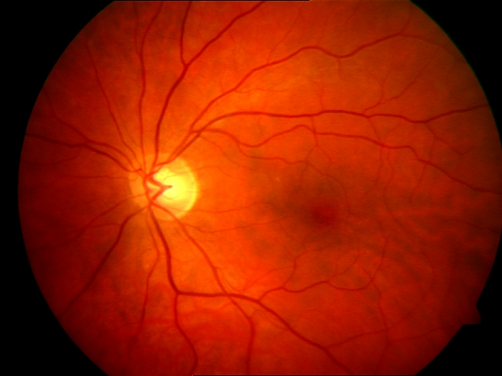
\includegraphics[height=2\textwidth]{./Figures/imagesARIA.png}\hspace{10mm}
        \caption{Aria}
        \label{fig:Aria}
    \end{subfigure}
    \begin{subfigure}[b]{0.1\textwidth}
				\centering
        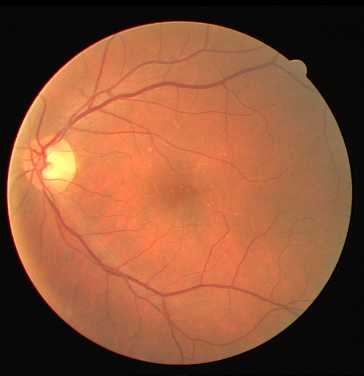
\includegraphics[height=2\textwidth]{./Figures/imagesDRIVE.png}\hspace{10mm}
        \caption{Drive}
        \label{fig:Drive}
    \end{subfigure}
    \begin{subfigure}[b]{0.1\textwidth}
				\centering
        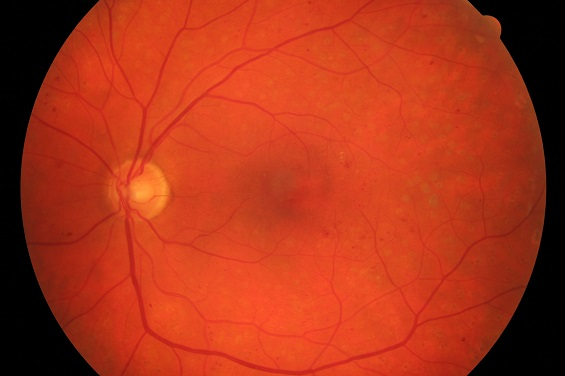
\includegraphics[height=2\textwidth]{./Figures/imagesHRF.png}\hspace{10mm}
        \caption{Hrf}
        \label{fig:Hrf}
    \end{subfigure}        
    \label{fig:Imagenes de fondo de ojo}
    \caption{(A) (B) (C)}
\end{figure}


Entre los beneficios clave est\'an la accesibilidad inmediata, visualizaci\'on, sistemas de gesti\'on de im\'agenes que permiten el seguimiento de la progresi\'on de la enfermedad mediante la revisi\'on de im\'agenes secuenciales, y la educaci\'on del paciente. Al mismo tiempo las im\'agenes capturadas, tienen una  gran resoluci\'on y se pueden visualizar en una pantalla tan pronto como se obtienen, permitiendo detectar y corregir cualquier error en el proceso fotogr\'afico a la vez. \cite{cunha2004blood}
Esta modalidad presenta determinadas ventajas al momento de compararla con las modalidades OCT y angiograf \'ia fluorescente. 
Ante la OCT la ventaja principal es el bajo costo del equipo necesario para realizar la captura en comparaci \'on con tom \'ografo necesario para tomar la OCT, y tambi \'en el tiempo de captura. En la OCT la captura demora entre 10 a 15’, mientras que la imagen de fondo de ojo se obtiene instant \'aneamente. Tambi \'en se puede considerar como una ventaja la portabilidad del equipo encargado de la captura, ya que hoy en d \'ia se han diseñado oftalmoscopios pequeños, de modo que sean acoplables a la c \'amara de un celular o c \'amara digital convencional, permitiendo transportar el equipo para poder alcanzar poblaciones en riesgo para analizar el estado de salud de su retina, algo que no se podr \'ia realizar con facilidad con un tom \'ografo retinal.
Al momento de compararla con la modalidad angiograf \'ia con florescencia, las ventajas que encontramos son el bajo costo del dispositivo de captura. En las im \'agenes de fondo de ojo, como se menciono, se utiliza una c \'amara digital convencional, en cambio para la angiograf \'ia se requiere de una c \'amara m \'as costosa, que sea capaz de capturar el espectro de luz que irradia la sustancia fluorescente inyectada en el paciente. La ventaja mas significativa en esta comparaci \'on es que la modalidad de angiograf \'ia fluorescente es invasiva, ya que requiere la inyecci \'on de una sustancia fluorescente, mientras que para obtener las im \'agenes de fondo de ojo no.

A continuaci\'on se puede observar las distintas partes del ojo en una imagen de fondo de ojo:
\begin{figure}[H]
	{
	\centering
	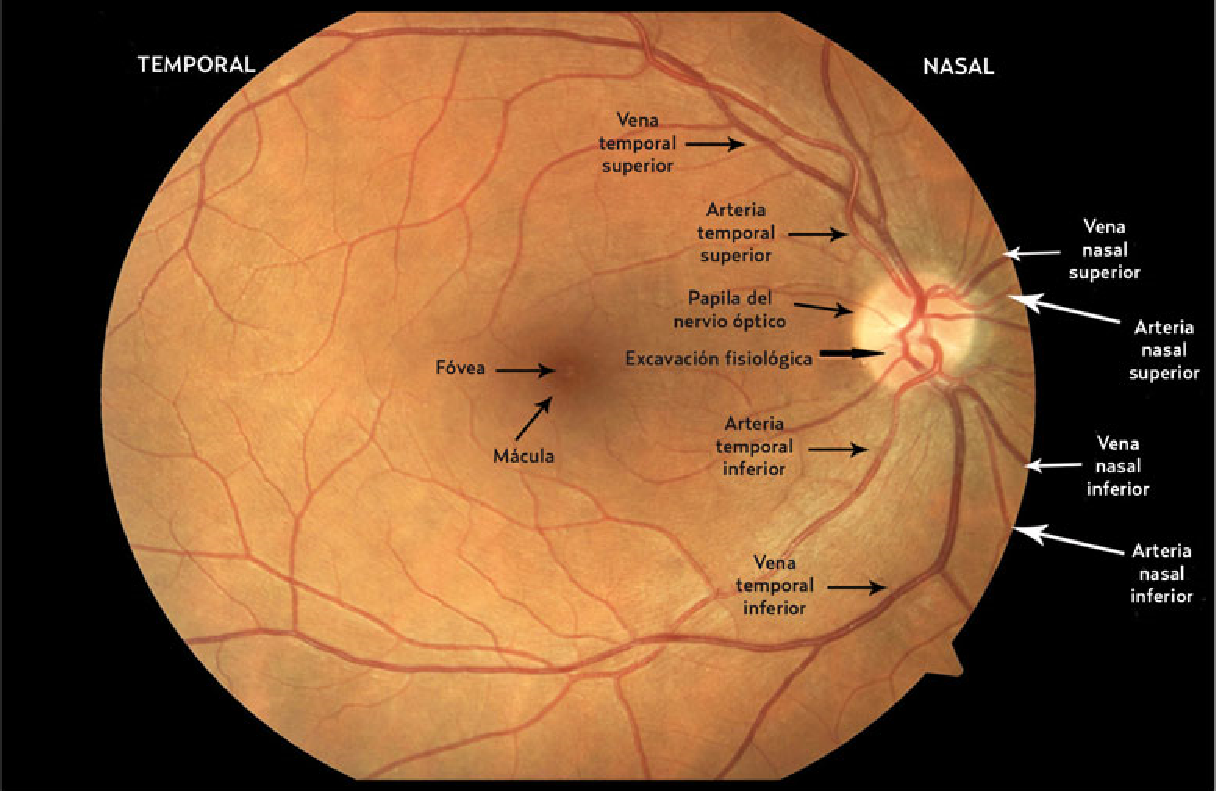
\includegraphics[width=0.75\textwidth]{Figures/ComposicionOjoIFO}
	\caption[Glaucoma]{Composici\'on del ojo en una im\'agen de fondo de ojo}
	\label{fig:Composici\'on del ojo, observada en una im\'agen de fondo de ojo}
	}
\end{figure}

As\'i como permiten identificar las distintas secciones del \'organo ocular, tambi\'en esta modalidad permite identificar estructuras patol\'ogicas ocasionadas por alguna determinada enfermedad:
\begin{figure}[H]
	{
	\centering
	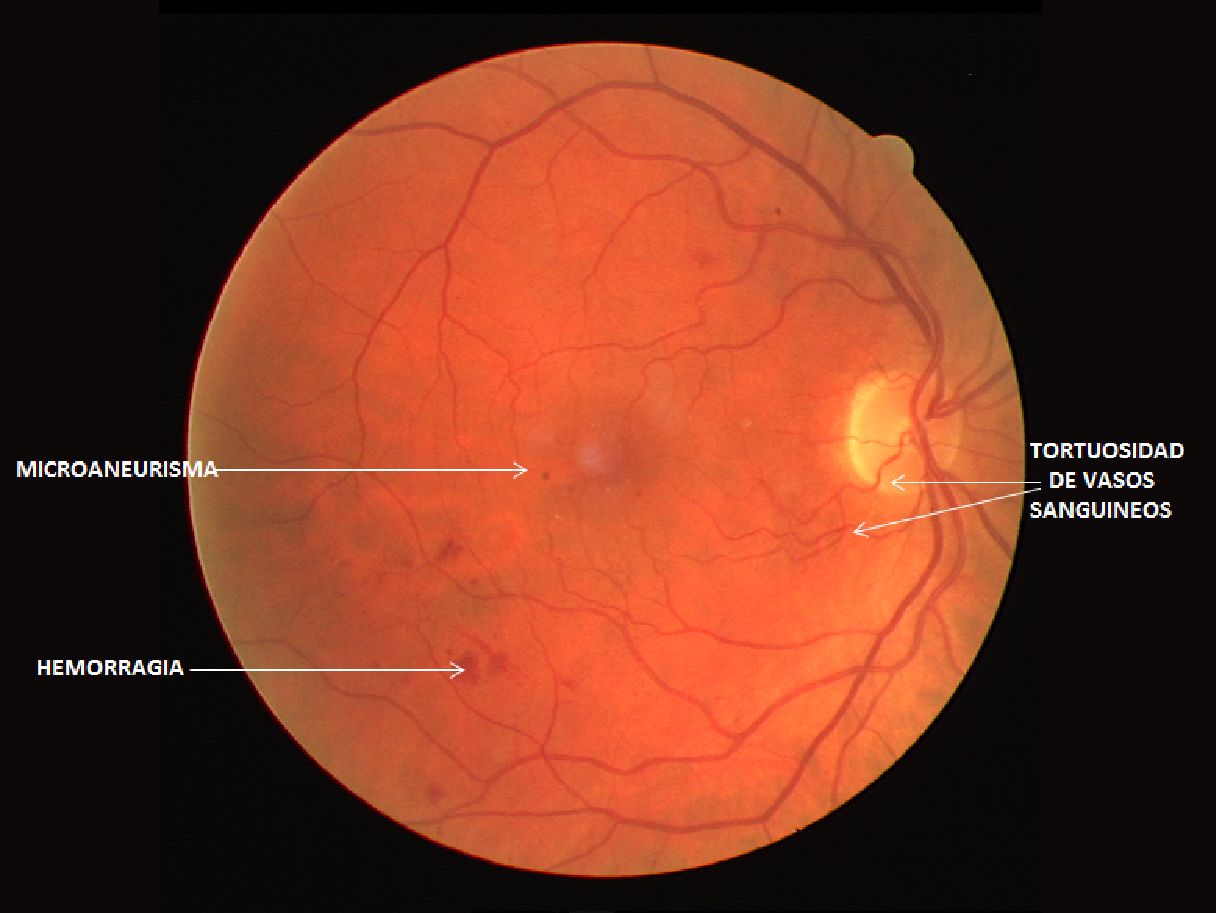
\includegraphics[width=0.5\textwidth]{Figures/HMT}
	\caption[HMT]{Hemorragias,microaneurisma y tortuosidad de vasos sangu\'ineos}
	\label{fig:Hemorragias,microaneurisma y tortuosidad de vasos sangu\'ineos}
	}
\end{figure}

\begin{figure}[H]
	{
	\centering
	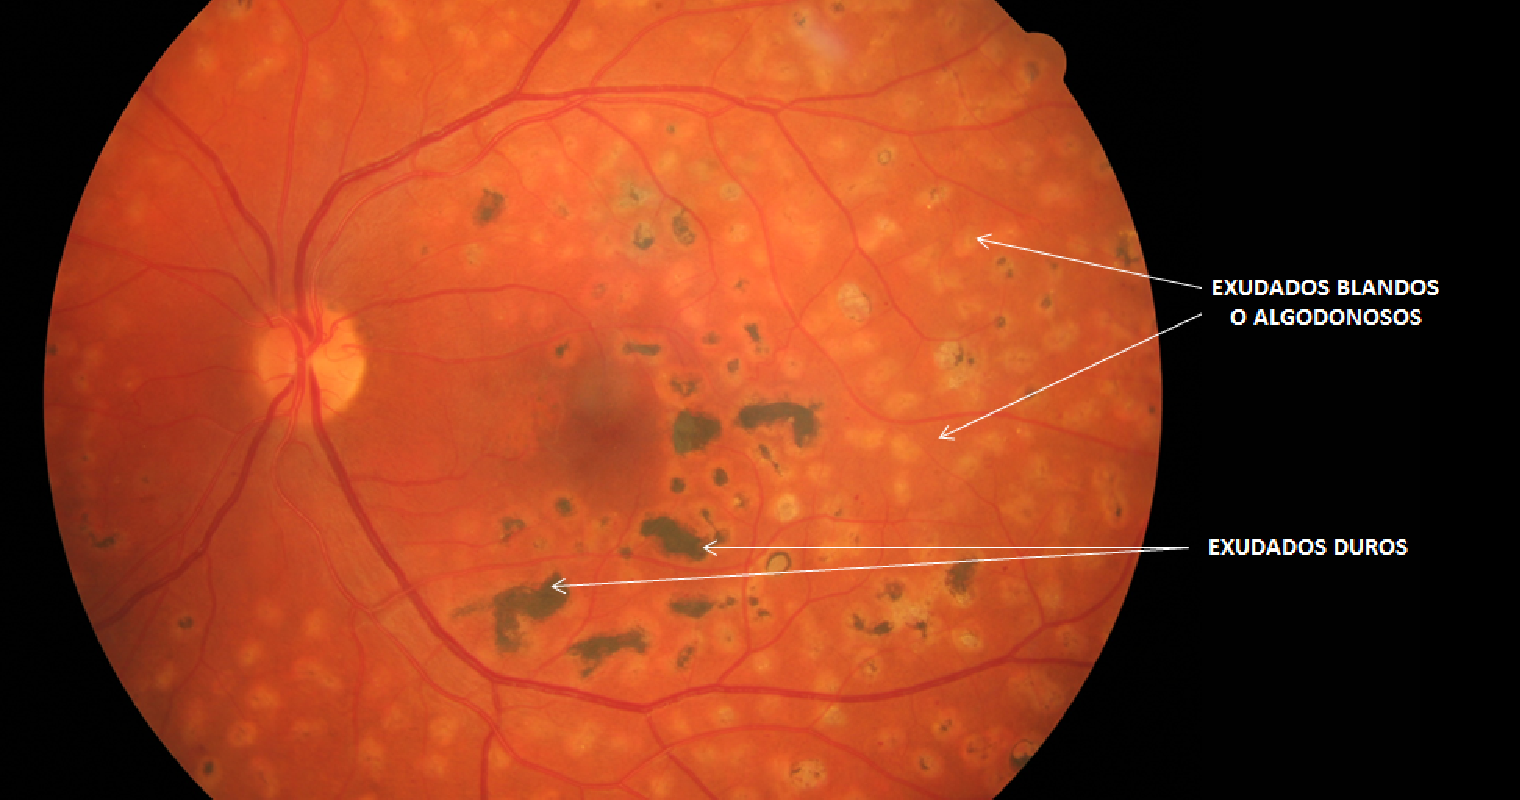
\includegraphics[width=0.5\textwidth]{Figures/EDyB}
	\caption[Exudados]{Exudados blandos o algodonosos y duros}
	\label{fig:Exudados blandos o algodonosos y duros}
	}
\end{figure}

\begin{figure}[H]
	{
	\centering
	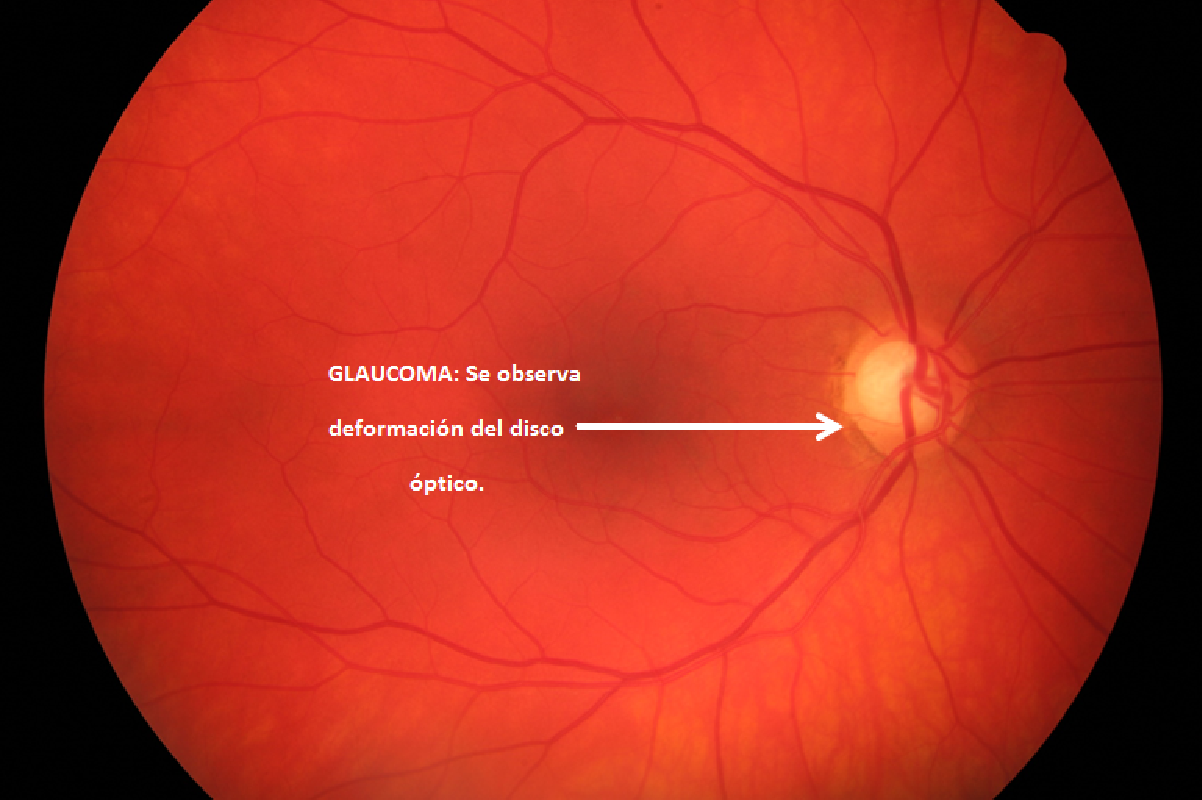
\includegraphics[width=0.5\textwidth]{Figures/Glaucoma}
	\caption[Glaucoma]{Glaucoma}
	\label{fig:Ojo afectado por Glaucoma.}
	}
\end{figure}

As\'i como mencionamos las ventajas de la modalidad de fondo de ojo frente a las modalidades OCT y la angiograf\'ia fluorescente, tambi\'en existen algunas desventajas en la comparaci\'on entre estas. Respecto a la OCT, es que esta \'ultima ofrece una vista en 3D del \'organo ocular, mientas que la imagen de fondo de ojo ofrece una visi\'on 2d. Y comparado con la angiograf\'ia fluorescente, la principal diferencia, es que es la angiograf\'ia permite visualizar con mayor claridad los vasos sangu\'ineos, gracias al agente fluorescente inyectado en el paciente.
Utilizando las im\'agenes de fondo de ojo se pueden detectar hemorragias, exudados duros y blandos, microaneurismas y identificar la tortuosidad de los vasos sangu\'ineos, permitiendo detectar la presencia de alguna enfermedad que presente alguna de estas estructuras patol\'ogicas, como la retinopat\'ia diab\'etica, la degeneraci\'on macular asociada a la edad y el glaucoma.
%-----------------------------------
%	SUBSECTION 3
%-----------------------------------

\subsection{Herramientas computacionales para an\'alisis de fotograf\'ias de fondo de ojo}

En el modo tradicional de diagn\'ostico, los oftalm\'ologos examinan las im\'agenes de la retina, buscan las posibles anomal\'ias que puedan llegar a existir y entregan un diagn\'ostico. El procesamiento y ana\'lisis autom\'atico de la retina permiten ahorrar carga de trabajo y ayudar a lograr una detecci\'on mas objetiva por parte de los oftalm\'ologos. Se han hecho esfuerzos para caracterizar de forma autom\'atica y robusta tanto estructuras anatómicas como patológicas en im\'agenes de la retina. La aplicaci\'on de t\'ecnicas de procesamiento de im\'agenes por computadora, para el an\'alisis de las im\'agenes de la retina comenz\'o aproximadamente hacia 1974 [1]. Desde entonces, muchos investigadores han presentado inter\'es en el tema, y han tenido que afrontar diversas dificultades, principalmente relacionadas con el ruido en las im\'agenes, iluminaci\'on desigual y la variaci\'on entre los individuos. \cite{li2004automated}
El uso de sistemas de im\'agenes digitales ha reducido la tasa de fallo t\'ecnico asociado con la fotograf\'ia de pel\'icula anterior no digital, y la imagen electr\'onica que permite un f\'acil almacenamiento y catalogaci\'on. Los sistemas digitales modernos utilizados en la fotograf\'ia de fondo de ojo han demostrado lograr una sensibilidad y especificidad de aproximadamente el 90\% en la detecci\'on de DR. (Lo anterior referencia a -> g0h2016)
En la actualidad para realizar el an\'alisis de un  estudio de fondo de ojo, se puede recurrir a la tecnolog\'ia, ya que la complejidad y la sobrecarga que puede sufrir el profesional pueden hacer de la tarea de an\'alisis algo complejo o imposible. Actualmente existe un gran volumen de informaci\'on generada por los distintos dispositivos de captura, y para lograr manipularlo podemos recurrir a la utilizaci\'on de distintas t\'ecnicas avanzadas de procesamiento, an\'alisis y visualizaci\'an de im\'agenes, como as\'i tambi\'en a la construcci\'on de modelos computacionales y de simulaci\'on.

El procesamiento de im \'agenes se divide en un conjunto de etapas, las cuales mencion \'aremos y describiremos a continuaci \'on:
1-	Captura de la imagen: en esta etapa se realiza la captura de la imagen.
2-	Pre procesamiento: en esta etapa se realiza un procesamiento de la imagen en donde se busca eliminar ruido o imperfecciones en la imagen. Estas pueden ser causadas por defectos en la c \'amara que realiza la captura, por un movimiento involuntario del paciente, part \'iculas en suspensi \'on, etc. Tambi \'en se busca realzar las estructuras propias del ojo, como la macula, vasos sangu \'ineos, etc.,  como as \'i tambi \'en las estructuras patol \'ogicas generadas por la presencia de alguna enfermedad, como por ejemplo hemorragias, exudados, etc. 
3-	Segmentaci \'on de estructuras anat \'omicas o patol \'ogicas: en este proceso se busca dividir la imagen digital en varias partes u objetos. El objetivo de la segmentación es simplificar y/o cambiar la representaci \'on de una imagen en otra m \'as significativa y m \'as f \'acil de analizar. La segmentaci \'on se usa tanto para localizar objetos como para encontrar los l \'imites de estos dentro de la imagen. M \'as precisamente, la segmentaci \'on de la imagen es el proceso de asignaci \'on de una etiqueta a cada p \'ixel de la imagen de forma que los p \'ixeles que compartan la misma etiqueta tambi \'en tendr \'an ciertas caracter \'isticas visuales similares. De esta forma se puede separar de la imagen la estructura de inter \'es, como pueden ser los vasos sangu \'ineos como se muestra en la FIGURAFIG.
4-	Caracterizaci \'on o cuantificaci \'on de las estructuras encontradas.
5-	Clasificación de las caracter \'isticas extra \'idas: De acuerdo a las caracter \'isticas encontradas se puede determinar si el ojo es sano o presenta alguna patolog \'ia.  

Dentro de las etapas del procesamiento de im\'agenes, un primer grupo de algoritmos se asocian con el pre-procesamiento y realce. Esta etapa puede resultar particularmente importante a fin de reducir el ruido o distorsiones que pueden afectar la informaci\'on presente en las im\'agenes, o para la extracci\'on de caracter\'isticas de inter\'es, seg\'un la aplicaci\'on en particular. Otro proceso importante es la segmentaci\'on, que permite la detecci\'on de diferentes estructuras dentro de la imagen y la construcci\'on de modelos geom\'etricos asociados, para su an\'alisis y visualizaci\'on, o sobre los cuales realizar la planificaci\'on y simulaci\'on de tratamientos. A partir de la informaci\'on obtenida de la imagen, por medio de estrategias de an\'alisis es posible reconocer patrones o extraer diferentes indicadores cuantitativos para evaluar la extensi\'on o distribuci\'on de una determinada estructura o patolog\'ia.
Entre otras aplicaciones, con este tipo de procesamientos se puede detectar, por ejemplo, una patolog\'ia en una imagen de fondo de ojo y analizar su variaci\'on en diferentes estadios de un tratamiento. Tambi\'en es posible extraer el \'arbol vascular o evidenciar estructuras patol\'ogicas y as\'i asistir en el diagn\'ostico y tratamiento de enfermedades, como la retinopat\'ia diab\'etica que puede provocar la reducci\'on o p\'erdida de la capacidad visual. Tambi\'en es factible la contribuci\'on al desarrollo de modelos personalizados de simulaci\'on para el estudio de enfermedades y su tratamiento.
 Esta digitalizaci\'on de los estudios y datos m\'edicos, conlleva al uso de sistemas de archivo y comunicaci\'on de im\'agenes conocidos como PACS (por Picture Archiving and Communication System), para la gesti\'on eficiente de las im\'agenes m\'edicas. Estos sistemas deben cumplir con el est\'andar DICOM (Digital Imaging and Communication of Medical Imaging) para su transmisi\'on y almacenamiento y con el est\'andar HL-7 (Health Level 7) para la transmisi\'on de datos m\'edicos, permitiendo la interconectividad de los equipos y terminales de trabajo, bajo determinados protocolos de seguridad.
Los aspectos más importantes en esta \'area se asocian a las telecomunicaciones, la inform\'atica m\'edica y los servicios de salud. Por medio de estos sistemas y est\'andares no solo es posible la interconexi\'on de los equipos y estaciones de trabajo en las instituciones de salud, sino que existe un creciente requerimiento de acceso remoto al PACS. Los desarrollos en este aspecto favorecen el avance de aplicaciones relacionadas con la telemedicina, o pr\'actica de servicios de medicina a distancia, a fin de obtener diagn\'osticos y segundas lecturas por parte de especialistas, proveer servicios radiol\'ogicos a sectores alejados de la poblaci\'on, entre otras posibilidades.

Esta utilizaci\'on y adaptaci\'on de la tecnolog\'ia en la medicina, se puede observar tambi\'en en la creaci\'on de sistemas o algoritmos destinados a realizar el diagn\'ostico de enfermedades de forma autom\'atica. Actualmente diversos desarrollos e investigaciones realizadas sobre este campo se han llevado a cabo, los cuales se centran en la detecci\'on de estructuras patol\'ogicas que presentan determinadas enfermedades de la retina. 
Para la detecci\'on de la retinopat\'ia diab\'etica en el trabajo de Thomas Walter y Jean-Claude Klein, se presento un sistema basado en la detecci\'on de exudados y el disco \'optico. Los exudados se encuentran mediante el uso de su variaci\'on del nivel de gris, y sus contornos están determinados por medio de t\'ecnicas de reconstrucci\'on morfol\'ogicas, y la detecci\'on del disco \'optico por medio de t\'ecnicas de filtrado morfol\'ogicas. \cite{walter2002contribution}.  En el trabajo de Timothy Spencer y  John Olson, presentan un sistema basado una transformaci\'on top-hat y el filtrado adaptativo para proporcionar una segmentaci\'on inicial de las im\'agenes. Luego se aplica una umbralaci\'on donde se obtiene una imagen binaria que contiene los microaneurismas candidatos, a continuaci\'on un nuevo algoritmo de regi\'on creciente delinea completamente cada objeto marcado. Posteriormente se realiza un an\'alisis del tamaño, forma, y la energ\'ia caracter\'istica de cada uno de los candidatos en la segmentaci\'on final de los microaneurismas. \cite{spencer1996image} .  En el trabajo de Meindert Niemeijer y Bram van Ginneken, presentan un sistema basado en aprendizaje, para detectar exudados y manchas algodonosas en fotograf\'ias del fondo de ojo digitales a color y diferenciarlos de drusas, para el diagn\'ostico precoz de la retinopat\'ia diab\'etica.\cite{frame1998comparison} \cite{niemeijer2007automated}
En lo que refiere a la detecci\'on autom\'atica de la degeneraci\'on macular asociada a la edad, en el trabajo de K. Rapantzikos y  M. Zervakis, se presenta un algoritmo de segmentaci\'on para la detecci\'on autom\'atica y mapeo de drusas en las im\'agenes de fondo de ojo. Aplican una ecualizaci\'on del histograma adaptativo modificado para mejorar las estructuras de intensidad locales. Para la detecci\'on de drusas en las im\'agenes de la retina, desarrollaron una t\'ecnica de segmentaci\'on, donde se obtiene el umbral basado en el histograma adaptativo local (HALT)\cite{rapantzikos2003detection}.En el trabajo de Carla Agurto y Simon Barriga, se presenta un algoritmo que clasifica autom\'aticamente las im\'agenes con las caracter\'isticas patol\'ogicas que se encuentran com\'unmente en la retinopat\'ia diab\'etica (RD) y la degeneraci\'on macular asociada a la edad (DMAE). Utilizan im\'agenes de segmentaciones conocidas y definidas (GROUND TRUE) para detectar la presencia de condiciones patol\'ogicas, incluyendo microaneurismas, hemorragias, exudados, neovascularización en el disco \'optico y en otros lugares, las drusas, pigmentaci\'on anormal, y la atrofia geogr\'afica \cite{agurto2011automatic}. En el trabajo de Cemal Köse y Uğur Şevik, se presenta un m\'etodo que extrae lesiones de la DMAE mediante el empleo de una m\'etodo estad\'istico. Este se utiliza primero para extraer el \'area sana de la m\'acula que es m\'as familiar y regular que las partes no saludables. Aqu\'i, las im\'agenes caracter\'isticas de los patrones de la m\'acula se extraen y se utilizan para segmentar las texturas sanas del ojo. Adem\'as de esto, los vasos sangu\'ineos son tambi\'en extra\'idos y despu\'es se clasifican como regiones sanas. Por \'ultimo, se genera una imagen inversa de la imagen segmentada, las cuales determinan las regiones insalubres de la m\'acula \cite{kose2010statistical} \cite{kose2008automatic}. 

Y con respecto a los sistemas automaticos de deteccion de glaucoma, se puede observar el trabajo de Jiang Liu y Damon Wing Kee Wong, donde se presenta un m\'etodo basado en el modelo estad\'istico para la segmentaci\'on del disco \'optico y la copa \'optica en im\'agenes de fondo de ojo. El m\'etodo combina Circular Hough Transform y una selecci\'on \'optima de canal para la segmentaci\'on del disco \'optico \cite{yin2012automated}. En el trabajo de Muthu Rama Krishnan Mookiaha y U. Rajendra Acharya, se presenta un sistema de identificaci\'on autom\'atica de clases normales y glaucoma utilizando espectros de orden superior (HOS) y la Transformada Wavelet Discreta caracter\'isticas (DWT). Las caracter\'isticas extra\'idas se utilizan como entrada para el clasificador de Apoyo Vector Machine (SVM) \cite{mookiah2012data}. En el trabajo de Rüdiger Bocka y Jörg Meier, presentan un m\'etodo que se centra en diferentes tipos de rasgos gen\'ericos que se comprimen mediante una t\'ecnica de reducci\'on de la dimensi\'on basada en la apariencia. Posteriormente, un esquema de clasificaci\'on de dos etapas probabil\'istico combina estos tipos de caracter\'isticas para extraer el \'indice de riesgo de Glaucoma \cite{bock2010glaucoma}. En el trabajo de Yanwu Xu y  Dong Xu, se define un m\'etodo que localiza autom\'aticamente la copa \'optica, que es la señal de imagen estructural primaria para identificar cl\'inicamente el glaucoma. Esta localizaci\'on utiliza un haz de ventanas din\'amicas de diferentes tamaños para obtener los discos \'opticos candidatos. A continuaci\'on  un modelo de vector de regresi\'on en base a la funci\'on de base radial no lineal, se utiliza para clasificar cada candidato \cite{xu2011sliding}.

%----------------------------------------------------------------------------------------
%	SECTION 2
%----------------------------------------------------------------------------------------

\section{Segmentaci\'on de vasos sangu\'ineos en im\'agenes de fondo de ojo}
La segmentaci\'on implica dividir las im\'agenes en subsecciones que son de particular inter\'es, tales como la definici\'on de \'areas de una imagen que sean apropiados para ser posteriormente analizadas, o la b\'usqueda de c\'irculos, l\'ineas u otras formas de inter\'es. Existen diversos algoritmos de segmentaci\'on para im\'agenes en escala de grises, los cuales se basan generalmente en la discontinuidad de las intensidades de la imagen tales como los bordes o en las similitudes. En la medicina, el objetivo es detectar tejidos o estructuras (anat\'omicas o patol\'ogicas) dentro de la imagen que se desean analizar seg\'un el problema o aplicaci\'on particular.

Es de gran importancia realizar una correcta segmentaci\'on de los vasos sangu\'ineos para el an\'alisis de las im\'agenes de fondo de ojo, ya que de esta dependen las etapas de representaci\'on, descripci\'on y extracci\'on de caracter\'isticas posteriores.  Tambi\'en es de suma importancia dado que permite detectar algunos cambios que se producen en la red de vasos sangu\'ineos se pueden considerar como indicios de ciertas enfermedades, como hemorragias y microaneurismas en la retinopat\'ia diab\'etica, por ejemplo. Por este motivo, cobra una gran importancia el desarrollo de herramientas que permitan segmentar esos vasos y que, en definitiva, ayuden al diagn\'ostico precoz de las enfermedades que afectan al ojo.

El presente trabajo final tiene por objetivo contribuir al desarrollo de un algoritmo que permita la extracci\'on eficaz y eficiente de los vasos sangu\'ineos. 
En la sección 2.2.1 presentaremos el rol que desempeña la segmentaci\'on en el diagnostico de enfermedades y mencionaremos investigaciones realizadas sobre este tema.  Tambi\'en realizaremos una breve descripci\'on de su utilidad para eliminar falsos positivos en algoritmos que detectan estructuras patol\'ogicas, definiremos y describiremos brevemente algunos algoritmos de registraci\'on basados en “landmarks” y algoritmos de identificaci\'on de personas a trav\'es en la distribuci\'on de los vasos sangu\'ineos del ojo.  A su vez enumeraremos las dificultades que se presentan en la segmentaci\'on manual. Finalmente presentaremos los m\'etodos de segmentaci\'on existentes hoy en d\'ia, describiendo su clasificaci\'on y en que consiste cada uno de ellos.



%-----------------------------------
%	SUBSECTION 1
%-----------------------------------

\subsection{Necesidad}
La evaluaci\'on de las caracter\'isticas de los vasos sangu\'ineos  juega un  rol central en el diagn\'ostico de diferentes enfermedades. En particular, ciertos indicadores tales como el grosor de los vasos, color, su reflectividad, tortuosidad, ramificaci\'on anormal, o la ocurrencia de los vasos de un cierto espesor  se relacionan con la existencia de algún tipo particular de enfermedad.
Por otro lado, el conocimiento acerca de la ubicación de los vasos puede ayudar
en la detección de patologías, por ejemplo, al reducir el número de falsos positivos
en la detección de microaneurismas o hemorragias (que presentan intensidades similares), o servir como un medio para el registro de imágenes
tomadas en diferentes instantes de tiempo o en diferentes lugares de la retina.\cite{staal2004ridge}
Cuando el n\'umero de vasos en una imagen es grande, o cuando se adquiere un gran n\'umero de im\'agenes, la segmentaci\'on manual de los vasos puede volverse tediosa o incluso imposible. 
Mediante m\'etodos computacionales, se puede realizar la segmentación autom\'aticamente, y utilizar la salida resultante como la entrada de una segunda herramienta de software que se encargue de  realizar un an\'alisis autom\'atico de la segmentaci\'on, y entregue la probabilidad de ocurrencia de alguna determinada patolog\'ia. De este modo, se puede etiquetar las im\'agenes que presenten una alta  probabilidad de presencia de alguna patolog\'ia retinal, para que sea analizada con m\'as detenimiento por un profesional. De este modo se puede acceder a poblaciones en riesgo, que no poseen acceso a un servicio de salud, permitiendo de esta manera realizar controles sin la necesidad del profesional presente, solo se requiere del dispositivo de captura. Esto permite encontrar a posibles pacientes en riesgo y derivarlos a un centro de salud para su atenci\'on. De igual manera, la salida de un algoritmo de segmentaci\'on puede utilizarse para...


Existen diferentes dificultades al momento de realizar el delineamiento de los vasos sangu\'ineos de modo manual por un oftalm\'ologo. Dado que si existe un gran numero de im\'agenes a las que se deben segmentar sus vasos sangu\'ineos o existe un gran numero de vasos en las im\'agenes, puede volver la tarea de segmentaci\'on sumamente tediosa o imposible. Adem\'as el delineamiento manual de los vasos sangu\'ineos, enfrenta el problema de que distintos profesionales generen segmentaciones distintas de una misma imagen. En cambio el procesamiento y ana\'lisis autom\'atico permiten ahorrar carga de trabajo y ayudar a lograr una detecci\'on mas objetiva por parte de los oftalm\'ologos. 
%-----------------------------------
%	SUBSECTION 2
%-----------------------------------

\subsection{M\'etodos existentes}
Segmentaci \'on Supervisada
Los algoritmos de segmentaci \'on supervisada necesitan de un conjunto de datos conocidos (etiquetados) para clasificar el universo de individuos. Son los llamados algoritmos con target conocido, los cuales, en base a un conocimiento a-priori de los segmentos de clasificaci \'on, clasifican el conjunto de datos. Se aplican t \'ecnicas de optimizaci \'on para el conjunto de individuos conocidos y se extrapola al universo de individuos no conocido. En este caso en particular, un algoritmo de segmentaci \'on supervisado significa que requiere de la segmentaci \'on realizada por otra herramienta o manualmente por un profesional, para poder comparar sus resultados con los que obtiene y validar la segmentación que obtuvo.

Segmentaci \'on No Supervisada
Los algoritmos de segmentaci \'on no supervisada se aplican cuando el conjunto de segmentos de clasificaci \'on no es conocido, y por tanto debe ser estimado sobre el universo completo de individuos. Se trata de algoritmos con un target desconocido, es decir, no se tiene conocimiento a-priori acerca del n \'umero o tipo de segmentos en los que se clasificar \'a el universo de individuos. Aplicado en este caso en particular, un algoritmo de segmentaci \'on no supervisado significa que no requiere de la segmentaci \'on realizada por otra herramienta o manualmente por un profesional, realizara  la segmentaci \'on en base a estimaciones que realice y en base a su definici \'on. Pero este tipo de algoritmos requiere de un tiempo mas prolongado para poder converger sus resultados, de modo que estos coincidan con una segmentaci \'on correcta de los vasos sangu \'ineos.


A continuaci\'on se describiran brevemente algunos de los m\'etodos de segmentaci\'on de vasos sangu\'ineos comunes que han sido reportados en la literatura reciente.
Se definir\'a cada m\'etodo y se discutir\'an sus ventajas y desventajas. Aunque cada t\'ecnica fue
creada separadamente, frecuentemente se utilizan m\'ultiples t\'ecnicas en conjunto con otras
para resolver diferentes problemas de segmentaci\'on.
Xu et al. [9], dividen los m\'etodos de segmentaci\'on de im\'agenes m\'edicas en 8
categor\'ias: m\'etodos de umbralado, m\'etodos de regi\'on creciente, clasificadores, m\'etodos
de agrupamiento (clustering methods), modelos de campos aleatorios de Markov, redes
neurales artificiales, modelos deformables y m\'etodos guiados por plantillas (atlasguided
methods). Al final de esta secci\'on se describen otros m\'etodos notables que no pertenecen a
ninguna de estas categor\'ias. De los m\'etodos mencionados anteriormente, los de
umbralado, clasificaci\'on, agrupamiento, y campos aleatorios de Markov, pueden
considerarse m\'etodos de clasificaci\'on de pixeles.
La mayor\'ia de los m\'etodos de segmentaci\'on que se describir\'an pueden ser vistos
como problemas de optimizaci\'on donde la segmentaci\'on deseada es la que minimiza alguna
funci\'on de energ\'ia o de costo, definida para una aplicaci\'on en particular. La ventaja de ver
la segmentaci\'on como un problema de optimizaci\'on es que define de manera precisa los
aspectos deseables de la segmentaci\'on. Es muy claro que, para diferentes aplicaciones, se
necesitan diferentes funciones de energ\'ia o costo. A continuaci\'on se explican brevemente:

\begin{itemize}
\item Umbralado: El umbralado (thresholding) es un m\'etodo que busca segmentar im\'agenes
escalares creando una partici\'on binaria de las intensidades de las im\'agenes. Un
umbralado trata de determinar un valor de intensidad, llamado umbral (threshold), que
separa la clases deseadas. La segmentaci\'on se logra agrupando todos los pixeles con mayor
Figura 2 (a) histograma de intensidades de grises en la imagen mostrando los posibles
umbrales (b) imagen en escala de grises intensidad al umbral en una clase, y todos los otros pixeles en otra clase.
\item Crecimiento de regiones: Crecimiento de regiones (region growing) es una t\'ecnica para extraer regiones de la imagen que est\'an conectadas seg\'un cierto criterio predefinido. Este criterio puede estar basado en
informaci\'on de intensidades y/o bordes de la imagen. En su forma más simple, este m\'etodo requiere un punto semilla (seed point) que es seleccionado manualmente por el usuario, y extrae todos los pixeles conectados a la semilla, que tengan el mismo valor de intensidad. Al igual que el umbralado, por lo general no se utiliza la regi\'on creciente solamente en una imagen, sino que se utiliza como parte de un conjunto de operaciones de procesamiento de im\'agenes, particularmente en la delineaci\'on de estructuras pequeñas y simples como tumores y lesiones. Su desventaja principal es que suele requerir interacci\'on manual para obtener el punto semilla. Los algoritmos de divisi\'on y mezcla (split and merge) están relacionados con la regi\'on creciente pero no requieren una semilla. En este caso, la segmentación se basa en... 
La regi\'on creciente tambi\'en puede ser sensible al ruido en la imagen y su resultado depende del o los parámetros relacionados con el criterio de crecimiento,esto puede causar que las regiones extra\'idas tengan agujeros e inclusive que se desconecten , requiriendo una etapa de post-procesamiento adicional.
\item Clasificadores: Los m\'etodos clasificadores son t\'ecnicas de reconocimiento de patrones que buscan particionar un espacio caracter\'istico derivado de la imagen usando datos con etiquetas conocidas. Un espacio caracter\'istico es un rango espacial de cualquier funci\'on de la imagen, siendo las intensidades de la imagen el m\'as com\'un de los espacios caracter\'isticos. Todos los pixeles cuyas caracter\'isticas est\'en en el lado derecho de la partici\'on ser\'ian agrupados en una clase.
Los clasificadores son conocidos como m\'etodos supervisados debido a que requieren datos de entrenamiento que son segmentados manualmente, para luego ser utilizados en la segmentaci\'on autom\'atica de nuevos datos.
\item Agrupamiento: Los algoritmos de agrupamiento (clustering) llevan a cabo esencialmente la misma
funci\'on que los m\'etodos clasificadores, pero sin utilizar datos de entrenamiento. Por lo tanto, son m\'etodos no supervisados. Para compensar la falta de los datos de entrenamiento, los m\'etodos de agrupamiento iteran entre segmentar la imagen y caracterizar las propiedades de cada clase. En este sentido, los m\'etodos de agrupamiento se entrenan a si mismos usando los datos disponibles. 
Aunque los algoritmos de agrupamiento no requieren que los datos se entrenen, si requieren un segmentaci\'on inicial (o de manera equivalente, requiere par\'ametros iniciales). Como los m\'etodos de clasificaci\'on, los algoritmos de agrupamiento no incorporan directamente un modelo espacial. De cualquier forma, esta falta de modelado espacial puede proveer ventajas significativas para realizar los c\'alculos velozmente. Es posible incorporar robustez al ruido usando campos aleatorios de Markov, como se describe en la sección siguiente.
\item Campos aleatorios de Markov: Los modelos de campos aleatorios de Markov (MRF – Markov Random Fields) no son un m\'etodo de segmentaci\'on en si mismos, pero son un modelo estad\'istico que puede ser usado dentro de los m\'etodos de segmentaci\'on. Los MRF modelan las interacciones espaciales entre vecinos o pixeles cercanos. Estas correlaciones locales proveen un Figura 4 (a) imagen original (b) segmentaci\'on usando el algoritmo de las K-medias mecanismo para modelar una variedad de propiedades de la imagen. En el tratamiento de im\'agenes m\'edicas, se utilizan frecuentemente para tomar en cuenta el hecho que la mayor\'ia de los pixeles pertenecen a la misma clase a la que pertenecen sus pixeles vecinos. En t\'erminos f\'isicos, esto implica que bajo la asunci\'on del MRF, cualquier estructura anat\'omica que consista de un solo p\'ixel tiene una probabilidad muy baja de ocurrir. Una dificultad asociada con los modelos MRF es la selección apropiada de los par\'ametros que controlan la fuerza de las interacciones espaciales. Una selecci\'on muy alta puede resultar en segmentaci\'on excesivamente suave y una p\'erdida de los detalles estructurales. En adici\'on, los m\'etodos MRF usualmente requieren algoritmos computacionalmente intensivos. A pesar de estas desventajas, los MRF son ampliamente utilizados no solo para modelar clases de segmentaci\'on, sino tambi\'en para modelar propiedades de texturas e inhomogenidades de las intensidades.
\item Redes Neurales Artificiales: Las Redes Neurales Artificiales (ANN – Artificial Neural Network) son redes masivamente paralelas de procesamiento de elementos o nodos que simulan el aprendizaje
biol\'ogico. Cada nodo en una ANN es capaz de llevar a cabo c\'alculos elementales. Las ANN representan un paradigma para el aprendizaje de las m\'aquinas y pueden ser usadas en una variedad de formas de segmentaci\'on de im\'agenes. El uso que m\'as se le da en procesamiento de im\'agenes m\'edicas es el de un clasificador, donde los pesos son determinados usando datos de entrenamiento y luego se utiliza la ANN para segmentar nuevos datos. Las ANN tambi\'en pueden ser usadas de una manera no supervisada como m\'etodo de agrupamiento o como modelo deformable. Debido al gran n\'umero de interconexiones utilizadas en un red neural, se puede incorporar f\'acilmente informaci\'on espacial en los procedimientos de clasificaci\'on. Aunque las ANN son inherentemente paralelas, pero frecuentemente se implementan en computadores seriales, y esto reduce su potencial computacional.
\item Modelos deformables: Los modelos deformables est\'an basados en motivaciones f\'isicas, utilizados para delinear bordes de regiones usando curvas o superficies param\'etricas cerradas que se deforman bajo la influencia de fuerzas externas e internas. De acuerdo al modelo original, para delinear el borde de un objeto en la imagen, se debe colocar una curva o superficie cerrada cerca del borde deseado y luego permitirle experimentar un proceso iterativo de relajación. Las fuerzas internas se se asocian a propiedades de la curva o superficie para mantenerla suave a lo largo de la deformaci\'on. Las fuerzas externas son frecuentemente derivadas de la imagen para llevar la curva o superficie hacia la caracter\'istica de inter\'es deseada.
\item Guiados por plantillas: Los m\'etodos guiados por plantillas (atlasguided methods) son una poderosa
herramienta para la segmentación de im\'agenes m\'edicas cuando esta disponible una plantilla o mapa est\'andar. El mapa o plantilla es generada por informaci\'on compilada de la anatom\'ia que requiere segmentaci\'on. Este mapa es utilizado como un marco de referencia para segmentar nuevas im\'agenes. Conceptualmente, los m\'etodos guiados por plantillas son similares a los clasificadores con la excepci\'on de que est\'an implementados en el dominio espacial de la imagen en lugar de en un espacio caracter\'istico.
\item Otros m\'etodos: Otro m\'etodo de segmentaci\'on es el de ajuste al modelo (model-fitting) que por lo general consiste en tratar de ajustar un forma geom\'etrica simple, como una elipse o par\'abola, a la localizaci\'on de caracter\'isticas de la imagen. Es una t\'ecnica que debe especializarse para la estructura que se segmenta pero se implementa f\'acilmente y puede proveer buenos resultados cuando el modelo es apropiado. Una t\'ecnica m\'as general es ajustar superficies o curvas spline, como en el trabajo de Rueckert et. al. [6]. La dificultad principal con el model-fitting es que las caracter\'isticas de la imagen deben ser extra\'idas antes de realizar el ajuste. El algoritmo de watershead usa conceptos de matem\'atica morfol\'ogica para particionar la imagen en regiones homog\'eneas. Este m\'etodo sufre de sobresegmentaci\'on, la cual ocurre cuando la imagen es segmentada en un n\'umero innecesario de regiones. Por lo tanto, los algoritmos de watershead en im\'agenes médicas por lo general son procesados posteriormente para mezclar regiones separadas que pertenecen a la misma estructura. \cite{coto2003metodos}
\end{itemize}
